\documentclass{article}
\usepackage{geometry}

\usepackage[english]{babel}
\usepackage{subcaption}
\usepackage{amsthm}
\usepackage{amsmath}
\usepackage{amssymb}
\usepackage{mathtools}
\usepackage{tikz-cd}
\usepackage{tikz}
\usetikzlibrary{decorations.markings}
\usetikzlibrary{calc}
\usepackage{trimclip}
\usepackage{xcolor}

\usepackage{xspace}

\usepackage{url}
\definecolor{pastelblue}{RGB}{0,72,205}
\usepackage[hidelinks]{hyperref}
\hypersetup{
 colorlinks,
 linktoc=page,
 linkcolor=pastelblue,
 citecolor=pastelblue,
 urlcolor=pastelblue
}
\usepackage[capitalise,noabbrev]{cleveref}
\usepackage{url}

\captionsetup[subfigure]{subrefformat=simple,labelformat=simple}
\renewcommand\thesubfigure{(\alph{subfigure})}

\newcommand{\kevin}[1]{\textcolor{violet}{\textbf{Kevin}: #1}}
\newcommand{\juli}[1]{\textcolor{orange}{\textbf{Juli}: #1}}

%opening
\title{Generalizing Isabelle's Lifting Package}
\date{}
\author{Juli Gottfriedsen}


\theoremstyle{definition}
\newtheorem{definition}{Definition}[section]
\newtheorem{theorem}[definition]{Theorem}
\newtheorem{lemma}[definition]{Lemma}
\newtheorem{corollary}[definition]{Corollary}
\newtheorem{example}[definition]{Example}

\mathchardef\mhyphen="2D

\newcommand{\cleftsemicirc}{\put(3.5,2.5){\oval(4,4)[l]}\put(3.5,.5){\line(0,1){4}}\phantom{\circ}}
\newcommand{\crightsemicirc}{\put(1.5,2.5){\oval(4,4)[r]}\put(1.5,.5){\line(0,1){4}}\phantom{\circ}}
\newcommand{\newcirc}{\put(1.5,2.5){\circle{3.4}}\phantom{\circ}}

\newcommand{\relfuncomp}{\mathbin{\circ\hspace{0.1ex}\clipbox*{0.55ex 0pt 1.5ex 1.5ex}{\(\circ\)}\hspace{-0.35ex}}}
\newcommand{\funrelcomp}{\mathbin{\hspace{-0.75ex}\clipbox*{0pt 0pt 0.55ex 1.5ex}{\(\circ\)}\hspace{0.1ex}\circ}}

\newcommand{\relcomp}{\mathbin{\circ\circ}}
\newcommand{\inv}{^{-1}}
\newcommand{\indom}{\mathsf{in\mhyphen{}dom}}
\newcommand{\incodom}{\mathsf{in\mhyphen{}co\mhyphen{}dom}}
\newcommand{\dom}{\mathsf{dom}}
\newcommand{\codom}{\mathsf{co\mhyphen{}dom}}
\newcommand{\bool}{\mathsf{Bool}}
\newcommand{\eq}{\mathsf{Eq}}
\newcommand{\eqrep}{\mathsf{Eq_{rep}}}
\newcommand{\eqabs}{\mathsf{Eq_{abs}}}
\newcommand{\id}{\mathsf{id}}
\newcommand{\mapfun}{\mathsf{map_\Rightarrow}}
\newcommand{\relfun}{\mathsf{Rel_\Rightarrow}}
\newcommand{\mapfund}{\mathsf{map_{\Rightarrow d}}}
\newcommand{\rel}{\mathsf{Rel}}
\newcommand{\relfund}{\mathsf{Rel_{\Rightarrow d}}}
\newcommand{\bijection}{\mathsf{bijection}}
\newcommand{\birel}{\mathsf{Bi\mhyphen{}Rel}}
\newcommand{\univ}{\mathsf{Univ}}
\newcommand{\snd}{\mathsf{snd}}
\newcommand{\nat}{\mathbb{N}}
\newcommand{\inte}{\mathbb{Z}}
\newcommand{\rat}{\mathbb{Q}}
\newcommand{\abs}{\mathsf{abs}}
\newcommand{\rep}{\mathsf{rep}}
\newcommand{\mapsum}{\mathsf{map_+}}
\newcommand{\mapprod}{\mathsf{map_\times}}
\newcommand{\maplist}{\mathsf{map_\ast}}
\newcommand{\relsum}{\mathsf{rel_+}}
\newcommand{\relprod}{\mathsf{rel_\times}}
\newcommand{\rellist}{\mathsf{rel_\ast}}
\newcommand{\Left}{\mathsf{Left}}
\newcommand{\Right}{\mathsf{Right}}
\newcommand{\true}{\mathsf{True}}
\newcommand{\false}{\mathsf{False}}
\newcommand{\cons}{\mathbin{\#}}
\newcommand{\relint}{\mathsf{T_\inte}}
\newcommand{\appabs}{\mathsf{app_{abs}}}
\newcommand{\reland}{\mathsf{rel_\land}}
\newcommand{\maprel}{\mathsf{map_{rel}}}
\newcommand{\aprel}{\mathsf{ap_{rel}}}
\newcommand{\liftrel}{lifting relation\xspace}
\newcommand{\liftrels}{lifting relations\xspace}
\newcommand{\related}{\mathbin{\raisebox{-0.5pt}{$\centerdot$} \hspace{-2.9pt} \raisebox{3.5pt}{$\centerdot$}}}
\newcommand{\adj}{\mathsf{\boldsymbol{\cdot}}}

\definecolor{col1}{rgb}{0,0.5,0.7}
\definecolor{col2}{rgb}{0.9,0.4,0.0}

\bibliographystyle{plain}

\begin{document}

\maketitle
\begin{abstract}
The transfer and lifting packages of Isabelle/HOL
allow users to automatically translate statements and definitions between different types.
% and the lifting tool helps users to lift terms
% from one Pure-type to another one
% and provides rules about these terms for the transfer tool.
However, the latter is tailored to work with the static type system of Isabelle/Pure
and expects its transfer relations to be right-total and right-unique.
As such, it cannot be used to lift terms in a soft type systems,
as recently explored in Isabelle/Set.
We present a generalization of the lifting package that
relaxes the conditions put on its transfer relations and,
in particular,
allows users to lift terms between soft types.
We verified the theoretic foundations of our approach in Isabelle/HOL\footnote{The work of this paper can be found on \url{https://github.com/kappelmann/Isabelle-Set/tree/dec546894380c91344f5732e8cab7f49de28f4c4/Isabelle_Set/Transfer/restructured}}
and propose a new lifting algorithm.
\end{abstract}

\section{Introduction}
In Isabelle/HOL there are two widely used commands to construct new types from existing ones: \(\mathtt{typedef}\) and \(\mathtt{quotient\_type}\).
The former defines a new type from a subset and the latter from a quotient set of some type.
For instance, we can define the type \(\inte\) as a quotient of \(\nat \times \nat\) and the type of finite sets \(\alpha\ \mathsf{fset}\) as a subtype of \(\alpha\ \mathsf{set}\). Even though one type is defined as a subtype or quotient type of the other,
this relation is not captured by the type system.
In particular, one cannot apply functions operating on one type to values of the other type.
Similarly, theorems about one type are not directly applicable to the other one.
% Users do not want to reprove
% Moreover, while \(\inte\) is defined as a quotient type of \(\nat \times \nat\),
% from the perspective of a mathematician,

Rather than manually re-defining and re-proving
these definitions and statements,
users would prefer them to be automatically generated.
To do so, a framework capturing the correspondence between two types is needed.
Such frameworks are typically inspired by work of Reynolds~\cite{reynolds1983types}, Mitchel~\cite{mitchell1986representation}, and Wadler~\cite{wadler1989theorems},
and use relations for this purpose.
% The fundamental idea of relational parametricity is
% that we can model the connection between a pair of types as a set of pairs, i.e.\ a relation.
% We call such relations transfer relations.
% Every type which we do not want to translate is related to itself by the identity relation.
% The relation \(\mathsf{T}_{\nat, \inte} :: \nat \Rightarrow \inte \Rightarrow \bool\) relates each non-negative integer with the corresponding natural number and the relation \(\mathsf{T}_\inte :: \nat \times \nat \Rightarrow \inte \Rightarrow \bool\) relates each integer with all its representations.
For instance, we can express the connection between \(0_\nat\) and \(0_\inte\) as \(\mathsf{T}_{\nat, \inte}\ 0\ 0\) with a suitable relation \(\mathsf{T}_{\nat, \inte} :: \nat\Rightarrow\inte\Rightarrow\bool\).
% Given these relation, we can state facts like \(\mathsf{T}_{\nat, \inte}\ 0_\nat\ 0_\inte\) and \(\mathsf{T}_\inte\ (n+3, n)\ 3\).
% We call such rules \(T\ x\ y\), where \(T\) is a transfer relations, transfer rules.
Since type constructors like \((\Rightarrow)\) or \(\mathsf{set}\) and \(\mathsf{fset}\) map types to types, we express their connection by mappings from relations to relations. For instance, a function has type \(\alpha \Rightarrow \beta\) if it maps value of type \(\alpha\) to values of type \(\beta\),
and analogously, two functions are related by \(R \Rrightarrow S\) if they map inputs related by \(R\) to results related by \(S\).

% Inspired by the work of Mitchell on representation independence [ref],
The transfer tool~\cite{huffman2013lifting} of Isabelle/HOL allows one to translate theorems about one type to theorems about another type.
For example, it can translate between the statements
\begin{align*}
  \forall m\ n :: \nat\ldotp 0 < m \longrightarrow 0 < m * n,\\
\forall i\ j \in \{i :: \inte \mid 0 \leq i\}\ldotp 0 < i \longrightarrow 0 < i * j.
\end{align*}

While the transfer tool translates propositions,
the lifting tool~\cite{huffman2013lifting} lifts definitions from one type to another one.
For instance, it can lift the addition operator \(\mathsf{add_{\inte rep}}\ (m_1, n_1)\ (m_2, n_2) \coloneqq (m_1 + m_2, n_1 + n_2)\)
on the representation level of integers to the type
\(\inte \Rightarrow \inte \Rightarrow \inte\)
given that the user provides a respectfulness theorem that \(\mathsf{add_{\inte rep}}\) respects the equivalence classes of the quotient.

The transfer and lifting tools
work with the static type system of Isabelle/Pure.
This has many benefits:
every term has a unique type and types are automatically checked and inferred.
% However, static systems
However, the type system of Isabelle/Pure
does not support dependent types.
Moreover, it uses an coercive interpretation of
subtyping (where terms of a subtype need to be lifted with coercion functions)
rather than an inclusive one (in which $t : A$ and $A <: B$ implies $t : B$).
% Morever,
% However, as mentioned above,
% when one wants to refine a type to another one using a set of values,
% the operations and theorems of the original type are not applicable to new type and vise versa.
Soft types offer solutions to these problems,
as explored recently in Isabelle/Set~\cite{isabelleset}.
% In a soft type system, a type may be regarded as a predicate on terms.
% Operations and theorems can be reused between all soft types defined on a shared Pure-type.
% However, often a more expressive and flexible type system is desirable.
% For instance, with Pure-types, if one wants to encode a property like finiteness of sets in a type, one has to define a new type as .
% Since, from the perspective of the type system, these type are not related, operations defined on one type cannot be used for the other type. Similarly, the sematic connection between the types \(\nat\), \(\inte\) and \(\rat\) cannot be expressed in the HOL type system and hence theorems proven about \(\nat\) are not directly applicable to the set of non-negative integers.
% To some extend, one can use the Transfer- and Lifting-Tool to translate theorems and lift definitions from one type to another. This can, however become quiet cumbersome.
% This is becomes particularly useful when one takes the approach common in mathematics,
% encoding algebraic structures, datatypes, and even functions as sets.
% This way, the Pure-type system is of little use to prevent errors otherwise detected by a type checker.

While in some scenarios,
one can reduce the need of the lifting tool by using soft types instead of Pure-types,
% defined by the \(\mathtt{typedef}\) command,
there are still many applications to lift between soft types.
However, the lifting tool is designed to lift terms between Pure-types
and hence cannot be used directly.

In this paper,
we investigate the limitations of the lifting tool,
introduce a generalization of its theory,
and propose a new lifting algorithm applicable to soft types.
\cref{sec-prelims} introduces soft types and the theoretical foundations of the transfer and lifting tool.
In \cref{lift-trip-sec} we describe the limitations of the existing lifting tool
and generalize its theory appropriately.
Based on this, we propose a generalized lifting algorithm in \cref{sec:lift-alg}.
\cref{sec:appl} demonstrates the application of this algorithm in a set-theoretic framework.
Finally \cref{sec:concl} summarizes our work and outlines future work.

\section{Preliminaries}\label{sec-prelims}

\paragraph{Isabelle}
In Isabelle/Pure, the logical framework on which Isabelle/HOL~\cite{wenzel2021isabelle} is built on,
every term has a unique Pure-type. We state that a term \(t\) has the Pure-type \(\tau\) by \(t :: \tau\).
We write \(\sigma \Rightarrow \tau\) for the Pure-type of functions with domain \(\sigma\) and co-domain \(\tau\) .

\paragraph{Soft types}
Soft types allow users to encode (almost) arbitrary properties in a type.
Such a soft type is typically simply represented by a predicate.
If a term \(t\) has the soft type \(\tau\), we write \(t : \tau\).

In Isabelle/Set, the Pure-type of soft types is $\alpha\ \mathsf{type}$,
and the function \(\mathtt{type} :: (\alpha \Rightarrow \bool)\Rightarrow \alpha\ \mathsf{type}\) takes a predicate $P$ and returns a soft type such that
\(t : \mathtt{type}\ P\) if and only if \(P\ t\).
For instance, the soft type \(\mathtt{type}\ (\lambda i :: \inte\ldotp 0 \leq i)\) encodes the natural numbers within the Pure-type \(\inte\).
To further refine a soft type \(T\),
one can use the intersection type operator \((\&)\),
where \(x : T_1\  \&\  T_2\) if and only if \(x : T_1 \land x : T_2\).

Often, one wants do define a soft type inhabiting exactly the elements of a given set.
Formally, given a set $A$, one can specify such a type by \(\mathtt{type}\ (\lambda x\ldotp x \in A)\).
For ease of exposition, we silently drop this construction in this paper and simply write
$t : A$ to mean $t : \mathtt{type}\ (\lambda x\ldotp x \in A)$.

The final kind of soft type we use in this paper are dependent function types.
A function \(f\) has the soft type \((x : \sigma) \rightarrow \tau\ x\) if and only if \(\forall x\ldotp x : \sigma \longrightarrow f\ x : \tau\ x\).
If $\tau$ does not depend on its argument,
we use the simpler notation \(\sigma \rightarrow \tau\).
\newline

In the remainder of this section,
we introduce the two tools lifting and transfer from Isabelle/HOL.
We illustrate the idea of transfer relations and transfer rules
and how they are used by the transfer and lifting tool with a running example.
Assume we have a type \(\inte\) of integers and want to construct a type \(\rat\) of rationals.
We can construct \(\rat\) as a partial quotient of \(\inte \times \inte\).
More specifically, we can represent a rational number \(x\) as any pair \((i, j)\)
such that \(x \cdot j = i\),
where \(j \neq 0\).
When we define \(\rat\) in Isabelle/HOL as
\begin{equation*}
	\mathtt{quotient\_type}\ \rat = \inte \times \inte\, /\, \mathtt{partial} : \mathsf{R}_{\rat},
\end{equation*}
where
\begin{equation*}
	\mathsf{R}_\rat\ (i_1, j_1)\ (i_2, j_2) \coloneqq (\mathsf{mul_\inte}\ i_1\ j_2 = \mathsf{mul_\inte}\ i_2\ j_1) \land j_1 \neq 0 \land j_2 \neq 0,
\end{equation*}
we not only get the type \(\rat\)
but also the abstraction and representation functions
\(\abs_\rat :: \inte \times \inte \Rightarrow \rat\) and \(\rep_\rat :: \rat \Rightarrow \inte \times \inte\).
We can then define multiplication on $\mathbb{Q}$ as
\begin{equation}\label{eq:mul_rat}
	\mathsf{mul_\rat}\ x\ y \coloneqq \abs_\rat\ (\mathsf{mul_{\rat rep}}\ (\rep_\rat\ x)\ (\rep_\rat\ y)),
\end{equation}
where
\begin{equation*}
	\mathsf{mul_{\rat rep}}\ (i_1, j_1)\ (i_2, j_2) \coloneqq (\mathsf{mul_\inte}\ i_1\ i_2, \mathsf{mul_\inte}\ j_1\ j_2)\,.
\end{equation*}
If we manually want to prove symmetry of \(\mathsf{mul_\rat}\) by using
a proof that \(\mathsf{mul_{\rat rep}}\) is symmetric modulo \(\mathsf{R_\rat}\),
we have to unfold the definition of \(\mathsf{mul_\rat}\)
and apply elementary properties of \(\abs_\rat\).

In practice, one typically wants to define multiple abstract operations
using corresponding functions on the representation level and
derive theorems for these operations from the corresponding theorems on the representation level.
The process sketched above thus becomes rather repetitive.

\paragraph{Transfer tool} The transfer tool translates properties about abstract types to properties about the corresponding representation types.
It uses binary relations to express the connection between terms on the representation and abstraction level.
We follow the terminology of~\cite{huffman2013lifting}
and use the term \textit{transfer relation} for binary relations that serve the purpose of connecting representations and abstractions.
Binary relations are represented as binary predicates:
\begin{definition}[Binary relations]
	A binary relation $R$ is a function \(R :: \alpha \Rightarrow \beta \Rightarrow \mathsf{bool}\).
\end{definition}
For instance, the transfer relation \(\mathsf{T_\rat} :: \inte \times \inte \Rightarrow \rat \Rightarrow \bool\) can be defined as
\begin{equation}\label{eq:trans-rel-rat}
	\mathsf{T_\rat}\ x\ y \coloneqq \mathsf{R_\rat}\ x\ x \land (\abs_\rat\ x = y)\,.
\end{equation}
Since the pair of integers \((0, 1)\) is a representation of the rational number zero,
we can define \(\mathsf{zero_\rat}\coloneqq\abs_\rat\ (0, 1)\) and state the relatedness of these two terms as \(\mathsf{T_\rat}\ (0, 1)\ \mathsf{zero_\rat}\).
Any theorem of the form \(T\ x\ y\),
where \(T\) is a transfer relation,
is called a \emph{transfer rule}.
To relate \(\mathsf{mul_\rat}\) with \(\mathsf{mul_{\rat rep}}\),
it is not sufficient to have the transfer relation $\mathsf{T}_\rat$ between the argument and return types of these functions.
We also have to lift \(\mathsf{T}_\rat\) over the function type constructor.
Any function that lifts one or more transfer relations over a type constructor is called
a \emph{relator}.
Following~\cite{wadler1989theorems},
we define two functions
to be related if they map related arguments to related results:
\begin{equation*}
	\rel_\Rightarrow\ T_1\ T_2\ f\ g \coloneqq \forall x\ y\ldotp T_1\ x\ y \longrightarrow T_2\ (f\ x)\ (g\ y)\,.
\end{equation*}
We will also use the notation \(T_1 \Rrightarrow T_2\) for \(\relfun\ T_1\ T_2\), where \(\Rrightarrow\) is right associative.

Now, we can state the desired relatedness property:
\begin{equation*}
	(\mathsf{T_\rat} \Rrightarrow \mathsf{T_\rat} \Rrightarrow \mathsf{T_\rat})\ \mathsf{mul_{\rat rep}}\ \mathsf{mul_\rat}\,.
\end{equation*}
We can then register this transfer rule to the transfer tool.
Similarly, we can register rules that relate equality on \(\rat\) with \(\mathsf{R_\rat}\) on \(\inte \times \inte\) and universal quantification over \(\rat\) with bounded quantification over the set \(\mathsf{Dom_\rat} \coloneqq \{(i, j) \mid j \neq 0\}\).
This allows the transfer tool to translate the proof goal
\begin{equation*}
	\forall x\ y\ldotp \mathsf{mul_\rat}\ x\ y = \mathsf{mul_\rat}\ y\ x
\end{equation*}
to the goal
\begin{equation*}
	\forall x\ y \in \mathsf{Dom_\rat}\ldotp \mathsf{R_\rat}\ (\mathsf{mul_{\rat rep}}\ x\ y)\ (\mathsf{mul_{\rat rep}}\ y\ x)\,.
\end{equation*}

So far, we have seen
1) transfer relations between a representation and an abstraction version of a base type and
2) how to obtain new transfer relations by lifting transfer relations over a fixed type constructor.
The missing part deals with transfer relations between a representation and an abstraction version of a type constructor.

For example, consider the type definition of finite sets as a restriction of the type \(\mathsf{set}\):
\begin{equation*}
	\mathtt{typedef}\ \alpha\ \mathsf{fset} = \{S \mid \mathsf{finite}\ S\}
\end{equation*}
We define the corresponding transfer relation as \(\mathsf{T_{fset}}\ S\ F \coloneqq (S = \rep_\mathsf{fset}\ F)\). Note that this definition follows a simpler scheme then the definition of \(\mathsf{T_\rat}\) because \(\alpha\ \mathsf{fset}\) is a subtype while \(\rat\) is a partial quotient type.
We can also define two sets to be related
if for all elements in each of the sets,
there is a related element in the other one:
\begin{equation*}
	\mathsf{Rel_{set}}\ T\ A\ B \coloneqq (\forall x \in A\ldotp \exists y \in B\ldotp T\ x\ y) \land  (\forall y \in B\ldotp \exists x \in A\ldotp T\ x\ y)\,.
\end{equation*}
However, neither \(\mathsf{T_{fset}}\) nor \(\mathsf{Rel_{set}}\) on its own
is sufficient to relate terms of type \((\inte \times \inte)\ \mathsf{set}\) with terms of type \(\rat\ \mathsf{fset}\).
Instead, we have to compose the transfer relation \(\mathsf{T_{fset}}\) with the relator \(\mathsf{Rel_{set}}\)
to obtain a suitable parametrized transfer relation \(\mathsf{T_{fset p}}\ T \coloneqq \mathsf{Rel_{set}}\ T \relcomp \mathsf{T_{fset}}\)
with type \((\inte \times \inte)\ \mathsf{set} \Rightarrow \rat\ \mathsf{fset} \Rightarrow \bool \),
where $(\relcomp)$ is defined as follows:
\begin{definition}[Composition of binary relations]
	The composition of two binary relations \(R_1\) and \(R_2\) is written as \(R_1 \relcomp R_2\) and defined as
	\begin{equation}
		(R_1 \relcomp R_2)\ x\ y \coloneqq \exists z\ldotp R_1\ x\ z \land R_2\ z\ y.
	\end{equation}
\end{definition}

\paragraph{Lifting tool} Recall that the transfer tool translates properties between two types using transfer rules, which relate constants and operators on the representation and abstraction level by transfer relations.
Defining such transfer relations,
lifting the constants and operations on the representation level to the abstraction level,
and proving the transfer rules for these terms
is cumbersome but can in many cases be automated by the lifting tool.

More precisely, for any type defined by one of the commands \(\mathtt{typedef}\) or \(\mathtt{quotient\_type}\),
the lifting tool generates a transfer relation between the representation type and the newly defined abstract type.
If one defines a polymorphic type,
the tool also generates a relator.
Moreover, the tool can synthesize abstract terms from terms on the representation level and prove transfer rules for these terms,
which can then be used by the transfer tool.

Let us first have a close look at the commands \(\mathtt{typedef}\) and \(\mathtt{quotient\_type}\).
By writing \(	\mathtt{typedef}\ \tau = A\),
the former creates a \emph{subtype} \(\tau\) of $\sigma$ from a set \(A :: \sigma\ \mathsf{set}\).
If \(A = \mathsf{UNIV_\sigma}\)
then \(\tau\) is a \emph{type copy} of \(\sigma\).
The other command -- \(\mathtt{quotient\_type}\) -- allows us to construct quotient types.
To create a \emph{(total) quotient} type of some type \(\sigma\),
we can use the statement \(\mathtt{quotient\_type}\ \tau = \sigma\, /\, R\),
which prompts us to prove that \(R\) is an equivalence relation.
We can also define a \emph{partial quotient type} of \(\sigma\) using the command \(\mathtt{quotient\_type}\ \tau = \sigma\, /\, \mathtt{partial} : R\).
In this case,
we have to prove that \(R\) is a partial equivalence relation:
\begin{definition}[Partial equivalence relations]
  A binary relations \(R : \alpha \Rightarrow \alpha \Rightarrow \bool\) is a \emph{partial equivalence relation} (PER) if it is symmetric and transitive. Formally, R must satisfy the property
	\begin{equation}
		(\forall x\ y\ldotp R\ x\ y \longleftrightarrow R\ y\ x) \land (\forall x\ y\ z\ldotp R\ x\ y \land R\ y\ z \longrightarrow R\ x\ z).
	\end{equation}
\end{definition}
Note that, if \(R : \alpha \Rightarrow \alpha \Rightarrow \bool\) is a PER, then \(R\) is an equivalence relation on the part of \(\alpha\) on which \(R\) is reflexive.

% For the four kinds of types which we can construct with \(\mathtt{typedef}\) and \(\mathtt{quotient\_type}\) --
% type-copies and subtypes with former command and total and partial quotients with the latter --
\cref{fig:lift-tool-trans-rels} depicts examples of transfer relations that the lifting tool generates for these four kinds of type definitions.
For quotient types, the dotted blue circles visualize the equivalence classes of the PERs on the source type
and for subtypes and partial quotient types, the set of values that represent abstract values are highlighted in dashed orange ellipses.
Note that transfer relations for these cases are always right-total and right-unique.

\begin{figure}[h]
	\centering
	\begin{subfigure}[b]{0.4\textwidth}
		\centering
		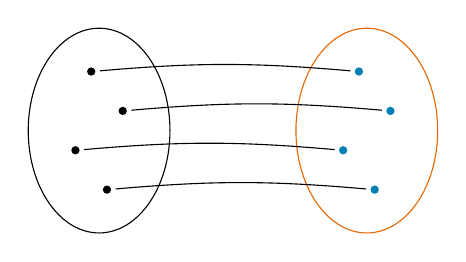
\begin{tikzpicture}
			\node[circle,fill=black,inner sep=0pt,minimum size=3pt] (r1) at (-1.8,1.5) {};
			\node[circle,fill=black,inner sep=0pt,minimum size=3pt] (r2) at (-1.4,1.0) {};
			\node[circle,fill=black,inner sep=0pt,minimum size=3pt] (r3) at (-2.0,0.5) {};
			\node[circle,fill=black,inner sep=0pt,minimum size=3pt] (r4) at (-1.6,0.0) {};
			\draw (-1.7, 0.75) ellipse (0.9cm and 1.3cm);
			\node[circle,fill=col1,inner sep=0pt,minimum size=3pt] (a1) at (1.6,1.5) {};
			\node[circle,fill=col1,inner sep=0pt,minimum size=3pt] (a2) at (2.0,1.0) {};
			\node[circle,fill=col1,inner sep=0pt,minimum size=3pt] (a3) at (1.4,0.5) {};
			\node[circle,fill=col1,inner sep=0pt,minimum size=3pt] (a4) at (1.8,0.0) {};
			\draw[col2] (1.7, 0.75) ellipse (0.9cm and 1.3cm);
			\path ($(r1.east)+(10:0.05)$) edge [-, bend left=5] ($(a1.west)+(170:0.05)$);
			\path ($(r2.east)+(10:0.05)$) edge [-, bend left=5] ($(a2.west)+(170:0.05)$);
			\path ($(r3.east)+(10:0.05)$) edge [-, bend left=5] ($(a3.west)+(170:0.05)$);
			\path ($(r4.east)+(10:0.05)$) edge [-, bend left=5] ($(a4.west)+(170:0.05)$);
		\end{tikzpicture}
		\caption{type copy}
	\end{subfigure}
	\hfill
	\begin{subfigure}[b]{0.4\textwidth}
		\centering
		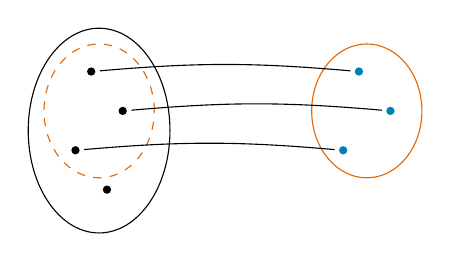
\begin{tikzpicture}
			\node[circle,fill=black,inner sep=0pt,minimum size=3pt] (r1) at (-1.8,1.5) {};
			\node[circle,fill=black,inner sep=0pt,minimum size=3pt] (r2) at (-1.4,1.0) {};
			\node[circle,fill=black,inner sep=0pt,minimum size=3pt] (r3) at (-2.0,0.5) {};
			\node[circle,fill=black,inner sep=0pt,minimum size=3pt] (r4) at (-1.6,0.0) {};
			\draw (-1.7, 0.75) ellipse (0.9cm and 1.3cm);
			\draw[dashed, col2] (-1.7, 1.0) ellipse (0.7cm and 0.85cm);
			\node[circle,fill=col1,inner sep=0pt,minimum size=3pt] (a1) at (1.6,1.5) {};
			\node[circle,fill=col1,inner sep=0pt,minimum size=3pt] (a2) at (2.0,1.0) {};
			\node[circle,fill=col1,inner sep=0pt,minimum size=3pt] (a3) at (1.4,0.5) {};
			\draw[col2] (1.7, 1.0) ellipse (0.7cm and 0.85cm);
			\path ($(r1.east)+(10:0.05)$) edge [-, bend left=5] ($(a1.west)+(170:0.05)$);
			\path ($(r2.east)+(10:0.05)$) edge [-, bend left=5] ($(a2.west)+(170:0.05)$);
			\path ($(r3.east)+(10:0.05)$) edge [-, bend left=5] ($(a3.west)+(170:0.05)$);
		\end{tikzpicture}
		\caption{subtype}
	\end{subfigure}
	\hfill
	\begin{subfigure}[b]{0.4\textwidth}
		\centering
		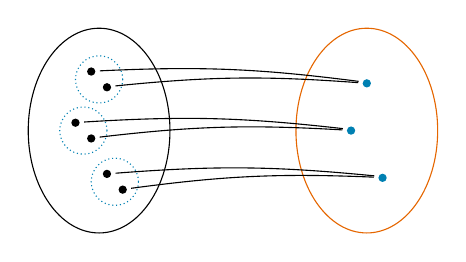
\begin{tikzpicture}
			\node[circle,fill=black,inner sep=0pt,minimum size=3pt] (r1) at (-1.8,1.5) {};
			\node[circle,fill=black,inner sep=0pt,minimum size=3pt] (r2) at (-1.6,1.3) {};
			\node[circle,fill=black,inner sep=0pt,minimum size=3pt] (r3) at (-2.0,0.85) {};
			\node[circle,fill=black,inner sep=0pt,minimum size=3pt] (r4) at (-1.8,0.65) {};
			\node[circle,fill=black,inner sep=0pt,minimum size=3pt] (r5) at (-1.6,0.2) {};
			\node[circle,fill=black,inner sep=0pt,minimum size=3pt] (r6) at (-1.4,0.0) {};
			\draw[densely dotted, col1] (-1.7, 1.4) ellipse (0.3cm and 0.3cm);
			\draw[densely dotted, col1] (-1.9, 0.75) ellipse (0.3cm and 0.3cm);
			\draw[densely dotted, col1] (-1.5, 0.1) ellipse (0.3cm and 0.3cm);
			\draw (-1.7, 0.75) ellipse (0.9cm and 1.3cm);
			\node[circle,fill=col1,inner sep=0pt,minimum size=3pt] (a1) at (1.7,1.35) {};
			\node[circle,fill=col1,inner sep=0pt,minimum size=3pt] (a2) at (1.5,0.75) {};
			\node[circle,fill=col1,inner sep=0pt,minimum size=3pt] (a3) at (1.9,0.15) {};
			\draw[col2] (1.7, 0.75) ellipse (0.9cm and 1.3cm);
			\path ($(r1.east)+(10:0.05)$) edge [-, bend left=5] ($(a1.west)+(150:0.05)$);
			\path ($(r2.east)+(20:0.05)$) edge [-, bend left=5] ($(a1.west)+(170:0.05)$);
			\path ($(r3.east)+(10:0.05)$) edge [-, bend left=5] ($(a2.west)+(150:0.05)$);
			\path ($(r4.east)+(20:0.05)$) edge [-, bend left=5] ($(a2.west)+(170:0.05)$);
			\path ($(r5.east)+(10:0.05)$) edge [-, bend left=5] ($(a3.west)+(150:0.05)$);
			\path ($(r6.east)+(20:0.05)$) edge [-, bend left=5] ($(a3.west)+(170:0.05)$);
		\end{tikzpicture}
		\caption{quotient type}
		\label{fig:trans-rels-quot}
	\end{subfigure}
	\hfill
	\begin{subfigure}[b]{0.4\textwidth}
		\centering
		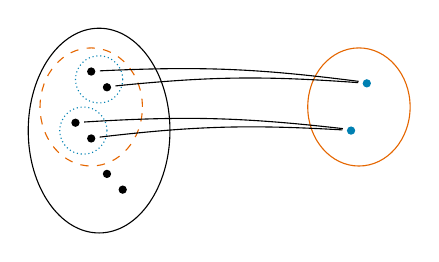
\begin{tikzpicture}
			\node[circle,fill=black,inner sep=0pt,minimum size=3pt] (r1) at (-1.8,1.5) {};
			\node[circle,fill=black,inner sep=0pt,minimum size=3pt] (r2) at (-1.6,1.3) {};
			\node[circle,fill=black,inner sep=0pt,minimum size=3pt] (r3) at (-2.0,0.85) {};
			\node[circle,fill=black,inner sep=0pt,minimum size=3pt] (r4) at (-1.8,0.65) {};
			\node[circle,fill=black,inner sep=0pt,minimum size=3pt] (r5) at (-1.6,0.2) {};
			\node[circle,fill=black,inner sep=0pt,minimum size=3pt] (r6) at (-1.4,0.0) {};
			\draw[densely dotted, col1] (-1.7, 1.4) ellipse (0.3cm and 0.3cm);
			\draw[densely dotted, col1] (-1.9, 0.75) ellipse (0.3cm and 0.3cm);
			\draw[dashed, col2] (-1.8, 1.05) ellipse (0.65cm and 0.75cm);
			\draw (-1.7, 0.75) ellipse (0.9cm and 1.3cm);
			\node[circle,fill=col1,inner sep=0pt,minimum size=3pt] (a1) at (1.7,1.35) {};
			\node[circle,fill=col1,inner sep=0pt,minimum size=3pt] (a2) at (1.5,0.75) {};
			\draw[col2] (1.6, 1.05) ellipse (0.65cm and 0.75cm);
			\path ($(r1.east)+(10:0.05)$) edge [-, bend left=5] ($(a1.west)+(150:0.05)$);
			\path ($(r2.east)+(20:0.05)$) edge [-, bend left=5] ($(a1.west)+(170:0.05)$);
			\path ($(r3.east)+(10:0.05)$) edge [-, bend left=5] ($(a2.west)+(150:0.05)$);
			\path ($(r4.east)+(20:0.05)$) edge [-, bend left=5] ($(a2.west)+(170:0.05)$);
		\end{tikzpicture}
		\caption{partial quotient type}
		\label{fig:trans-rels-par-quot}
	\end{subfigure}
	\caption{Visualization of transfer relations for type copies, subtypes, quotient types and partial quotient types.}
	\label{fig:lift-tool-trans-rels}
\end{figure}

In the remainder of this section,
we explain how the lifting tool synthesizes abstract terms from terms on the representation level.
For this purpose the tool provides the command \(\mathtt{lift\_definition}\).
With this command, we can, for instance, lift the term
\((0, 1)\) from \(\inte \times \inte\) to \(\rat\) and assign the name \(\mathsf{zero_\rat}\) to the lifted term:
\begin{equation*}
	\mathtt{lift\_definition}\ \mathsf{zero_\rat} :: \rat\ \mathtt{is}\ (0, 1)
\end{equation*}
Since we defined the type \(\rat\) as a partial quotient, the user must prove that the term \((0, 1)\) is indeed a representation of a rational.
This property is equivalent to the statement \(\mathsf{R_\rat}\ (0, 1)\ (0, 1)\).
Once we have discharged this obligation, the lifting tool defines \(\mathsf{zero_\rat}\) as \(\abs_\rat\ (0, 1)\).
Moreover, using \cref{eq:trans-rel-rat}, the lifting tool
proves the transfer rule \(\mathsf{T_\rat}\ (0, 1)\ \mathsf{zero_\rat}\).

Let us now generalize from this example:
We were able to prove \(\mathsf{T_\rat}\ (0, 1)\ \mathsf{zero_\rat}\) because the PER \(\mathsf{R_\rat}\),
the abstraction function \(\abs_\rat\),
and the transfer relation \(\mathsf{T_\rat}\)
stand in a particular relation to each other.
Before we can formalize this relation,
we need to define the inverse relation of a binary relation.
\begin{definition}[Inverse relations]
	The inverse of a binary relations \(R\) is written as \(R\inv\) and defined as
	\begin{equation}
		R\inv\ x\ y \coloneqq R\ y\ x.
	\end{equation}
\end{definition}

The quotient predicate~\cite{huffman2013lifting} is a tuple used by the lifting tool that formalizes said relationship between the PER on the source type,
the abstraction and representation functions,
and the transfer relation.
We will see later why it also has to include the representation function.
\begin{definition}[Quotient predicate~\cite{huffman2013lifting}]
  The terms \(R :: \alpha \Rightarrow \alpha \Rightarrow \bool\), \(abs :: \alpha \Rightarrow \beta\), \(rep :: \beta \Rightarrow \alpha\) and \(T :: \alpha \Rightarrow \beta \Rightarrow \bool\) form a \emph{quotient predicate},
  written \(\langle R, abs, rep, T \rangle\),
  if
	\begin{enumerate}
		\item \(R = T \relcomp T\inv\),
		\item \(\forall x\ y\ldotp T\ x\ y \longrightarrow abs\ x = y\), and
		\item \(\forall x\ldotp T\ (rep\ x)\ x\)\,.
	\end{enumerate}
\end{definition}
The third condition encapsulates two properties:
First, that the function \(rep\) respects the transfer relation \(T\) and second, that \(T\) is right-unique and right-total.
The second condition ensures that also the function \(\abs\) respects \(T\).
Lastly, the first condition states that two terms are related by \(R\) if and only if they are related to the same abstract term by \(T\).
Together with the fact that \(T\) is right-unique,
this guarantees that \(R\) is a PER.
While the lifting tool automatically proves quotient predicates for types defined by \(\mathtt{typedef}\) and \(\mathtt{quotient\_type}\),
users can also manually prove custom quotient predicates.

Now we can state the central theorem~\cite{huffman2013lifting} of the lifting tool that generalizes our reasoning why \(\mathsf{R_\rat}\ (0, 1)\ (0, 1)\) is valid:
\begin{equation}\label{eq:lifting-thm}
	\langle R, abs, rep, T \rangle \land abs\ x = y \land R\ x\ x \longrightarrow T\ x\ y
\end{equation}

Similarly to why we needed the function relator \(\rel_\Rightarrow\) in addition to the transfer relation \(\mathsf{T_\rat}\) to relate \(\mathsf{mul_{\rat rep}}\) with \(\mathsf{mul_\rat}\),
we have to lift the quotient predicate \(\langle \mathsf{R_\rat}, \abs_\rat, \rep_\rat, \mathsf{T_\rat} \rangle\) to the function space before we can lift \(\mathsf{mul_{\rat rep}}\) from the representation level to \(\rat \Rightarrow \rat \Rightarrow \rat\).
For the relations \(\mathsf{R_\rat}\) and \(\mathsf{T_\rat}\),
we can again use the relator \(\rel_\Rightarrow\).
To lift the functions \(\abs_\rat\) and \(\rep_\rat\) to the function space, we need a map function for the function type constructor.
Looking at \cref{eq:mul_rat},
we can see that we first applied the representation function to the arguments,
then applied the function on the representation level,
and finally applied the abstraction function to the result.
We hence define the map function for functions as
\begin{equation*}
	\mapfun\ f\ g\ h \coloneqq g \circ h \circ f.
\end{equation*}
With this, given quotient predicates \(\langle R_1, abs_1, rep_1, T_1 \rangle\) and \(\langle R_2, abs_2, rep_2, T_2 \rangle\) for the domain and co-domain, respectively,
we can build a new quotient predicate
\begin{equation}
	\langle \relfun\ R_1\ R_2, \mapfun\ rep_1\ abs_2, \mapfun\ abs_1\ rep_2, \relfun\ T_1\ T_2 \rangle\label{eq:fun-quot-pred}.
\end{equation}
Since the new quotient predicate involves the representation function of input quotient predicates,
we have to include both abstraction and representation functions in quotient predicates.
Applying this construction twice, we get the following PER, abstraction function,
and transfer relation:
\begin{align*}
	\mathsf{R}_{\rat \Rightarrow\rat \Rightarrow\rat} &\coloneqq \mathsf{R_\rat} \Rrightarrow \mathsf{R_\rat} \Rrightarrow \mathsf{R_\rat} \\
	\mathsf{map}_{\rat \Rightarrow\rat \Rightarrow\rat} &\coloneqq \mapfun\ \rep_\rat\ (\mapfun\ \abs_\rat\ \rep_\rat) \\
	\mathsf{T}_{\rat \Rightarrow\rat \Rightarrow\rat} &\coloneqq \mathsf{T_\rat} \Rrightarrow \mathsf{T_\rat} \Rrightarrow \mathsf{T_\rat}
\end{align*}
Using \cref{eq:lifting-thm},
we can prove \(\mathsf{T}_{\rat \Rightarrow\rat \Rightarrow\rat}\ \mathsf{mul_{\rat rep}}\ (\mathsf{map}_{\rat \Rightarrow\rat \Rightarrow\rat}\ \mathsf{mul_{\rat rep}})\) given a proof
of the respectfulness theorem \(\mathsf{R}_{\rat \Rightarrow\rat \Rightarrow\rat}\ \mathsf{mul_{\rat rep}}\ \mathsf{mul_{\rat rep}}\).
With the right choice of map functions and relators, we can use similar constructions to lift quotient predicates over various type constructors, like lists and sets.

Note that if we want to lift, for instance,
the exponentiation function from \(\inte \times \inte \Rightarrow \nat \Rightarrow \inte \times \inte\) to \(\rat \Rightarrow \nat \Rightarrow \rat\),
where the type of the second parameter does not change,
% or a function like \((\leq) :: \bool \Rightarrow \bool\),
% where the result is \(\bool\) on both the representation and abstraction level,
we can use the identity quotient predicate \(\langle (=), \id, \id, (=) \rangle\).

As in above description of the transfer tool,
to account for the last case -- the lifting of type constructors --
we have to combine the previous lifting principles.
For this, we can use a composition theorem for quotient predicates~\cite{huffman2013lifting}:
\begin{theorem}\label{eq:quotient-comp}
	Given two quotient predicates \(\langle R_1, abs_1, rep_1, T_1 \rangle\) and \(\langle R_2, abs_2, rep_2, T_2 \rangle\), their composition \(\langle T_1 \relcomp R_2 \relcomp T_1\inv, abs_2 \circ abs_1, rep_1 \circ rep_2, T_1 \relcomp T_2 \rangle\) is a quotient predicate as well.
\end{theorem}
For example, lifting finite sets of rationals from \((\inte \times \inte)\ \mathsf{set}\) to \(\rat\ \mathsf{fset}\)
goes via the intermediate level \(\rat\ \mathsf{set}\). For this, we need the function \(\mathsf{map_{set}}\ f\ A \coloneqq \{f\ x \mid x \in A\}\).
Then we can prove
\begin{equation}
	\langle R, abs, rep, T\rangle \longrightarrow \langle \rel_\mathsf{set}\ R, \mathsf{map_{set}}\ abs, \mathsf{map_{set}}\ rep, \rel_\mathsf{set}\ T \rangle\label{eq:set-rel}\,.
\end{equation}
Applying this to \(\langle \mathsf{R_\rat}, \abs_\rat, \rep_\rat, \mathsf{T_\rat} \rangle\) and composing the result with \(\langle (=), \abs_\mathsf{fset}, \rep_\mathsf{fset}, \mathsf{T_{fset}} \rangle\) using \cref{eq:quotient-comp}, we get the quotient predicate required to lift terms from \((\inte \times \inte)\ \mathsf{set}\) to \(\rat\ \mathsf{fset}\).

\section{Lifting Relations and Lifting Triples}\label{lift-trip-sec}
As mentioned in \cref{sec-prelims},
the lifting tool only supports right-total, right-unique transfer relation.
Let us first demonstrate why this limitation is too restrictive,
in particular when working with soft types.
We then continue to explain how we can generalize the notion of transfer relations
and quotient predicates to support lifting for a wider range of use cases.

It is easy to see why transfer relation may not be right-total:
For instance, if we want to lift operations from \(\nat\) to $\inte$,
we need a transfer relation that relates natural numbers to
the non-negative subset of integers.
In Isabelle/HOL, we could use $\mathtt{typedef}$ to create a new Pure
type $\inte_+$ of that subset.
But this approach defeats the purpose and flexibility of a soft type system,
where terms of different types (such as $\nat$ and $\inte$)
may inhibit the same Pure-type $\mathsf{set}$.

To see why soft types can lead to non-right-unique transfer relations,
consider the two transfer relations on $\bool$ visualized in \cref{fig:bool-rels}:
The equality relation \((=)\) and equality restricted to the soft type \(\sigma \coloneqq \mathtt{type}\, ((=)\,\true)\),
which we denote \((=_\sigma)\).
Note that both relations are right-unique but the latter is not right-total.

\begin{figure}[ht]
	\centering
	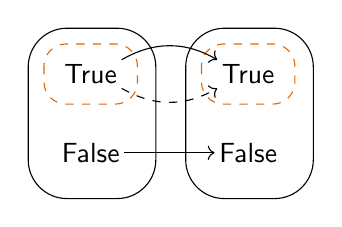
\begin{tikzpicture}
		\node[inner sep=1.5] at (-1,1) (tl) {$\true$};
		\node[inner sep=1.5] at (-1,0) (fl) {$\false$};
		\node[inner sep=1.5] at (1,1) (tr) {$\true$};
		\node[inner sep=1.5] at (1,0) (fr) {$\false$};
		\draw[rounded corners=8, dashed, col2] ($(tl.north west)+(-0.2,0.2)$)  rectangle ($(tl.south east)+(0.2,-0.2)$);
		\draw[rounded corners=8, dashed, col2] ($(tr.north west)+(-0.2,0.2)$)  rectangle ($(tr.south east)+(0.2,-0.2)$);
		\draw[rounded corners=14] ($(tl.north west)+(-0.4,0.4)$)  rectangle ($(fl.south east)+(0.4,-0.4)$);
		\draw[rounded corners=14] ($(tr.north west)+(-0.4,0.4)$)  rectangle ($(fr.south east)+(0.4,-0.4)$);
		\path (tl.north east) edge [->, bend left] (tr.north west);
		\path (tl.south east) edge [->, bend right, dashed] (tr.south west);
		\path (fl.east) edge [->] (fr.west);
	\end{tikzpicture}
	\caption{Transfer relations \((=)\) (solid arrows) and \((=_\sigma)\) (dashed arrow). The soft type \(\sigma\) is highlighted by the dashed orange border.}
	\label{fig:bool-rels}
\end{figure}

Now let us lift these transfer relations to the function space.
If we use \((=)\) for both the domain and co-domain, we get the right-unique, right-total transfer relation \((=) \Rrightarrow (=)\),
depicted in \cref{fig:bool-fun-rels} by solid arrows.
If, however, we use \((=_\sigma)\) for the domain,
we get the non-right-unique relation \((=_\sigma) \Rrightarrow (=)\),
visualized by the dashed arrows.
To see why this relation is not right-unique,
remember that two functions are related if they map related inputs to related results.
Since only \(\true\) is related to itself when using \((=_\sigma)\),
but \(\false\) is not related to anything,
two functions are related by \((=_\sigma) \Rrightarrow (=)\) if and only if they map \(\true\) to the same value.
% In other words, it is not relevant, what \(\false\) is mapped to.
% This in particular means that all functions at the right side of \cref{fig:bool-fun-rels}
% that behave equivalently on the soft type \(\sigma\)
% are related to the same function on the left side.
% The resulting PERs are highlighted with dotted blue borders in \cref{fig:bool-fun-rels}.

\begin{figure}[h]
	\centering
	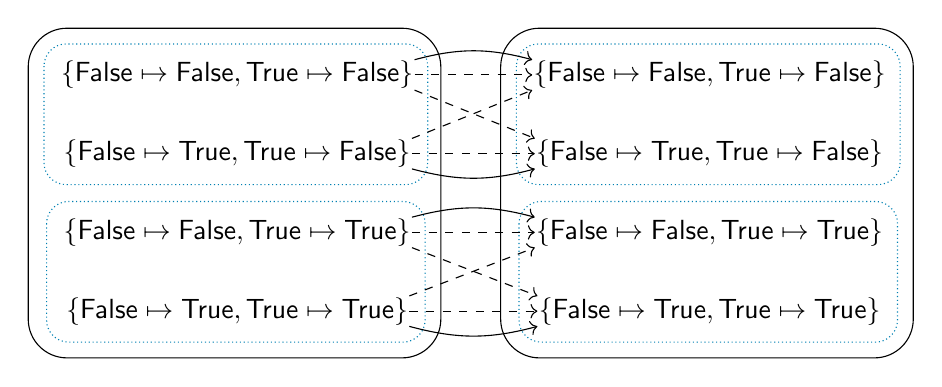
\begin{tikzpicture}
		\node[inner sep=0.3] at (-3,3) (l1) {$\{\false \mapsto \false, \true \mapsto \false\}$};
		\node[inner sep=0.3] at (-3,2) (l2) {$\{\false \mapsto \true, \true \mapsto \false\}$};
		\node[inner sep=0.3] at (-3,1) (l3) {$\{\false \mapsto \false, \true \mapsto \true\}$};
		\node[inner sep=0.3] at (-3,0) (l4) {$\{\false \mapsto \true, \true \mapsto \true\}$};
		\node[inner sep=0.3] at (3,3) (r1) {$\{\false \mapsto \false, \true \mapsto \false\}$};
		\node[inner sep=0.3] at (3,2) (r2) {$\{\false \mapsto \true, \true \mapsto \false\}$};
		\node[inner sep=0.3] at (3,1) (r3) {$\{\false \mapsto \false, \true \mapsto \true\}$};
		\node[inner sep=0.3] at (3,0) (r4) {$\{\false \mapsto \true, \true \mapsto \true\}$};
		\draw[rounded corners=8, densely dotted, col1] ($(l1.north west)+(-0.2,0.2)$)  rectangle ($(l2.south east)+(0.2,-0.2)$);
		\draw[rounded corners=8, densely dotted, col1] ($(l3.north west)+(-0.2,0.2)$)  rectangle ($(l4.south east)+(0.2,-0.2)$);
		\draw[rounded corners=8, densely dotted, col1] ($(r1.north west)+(-0.2,0.2)$)  rectangle ($(r2.south east)+(0.2,-0.2)$);
		\draw[rounded corners=8, densely dotted, col1] ($(r3.north west)+(-0.2,0.2)$)  rectangle ($(r4.south east)+(0.2,-0.2)$);
		\draw[rounded corners=14] ($(l1.north west)+(-0.4,0.4)$)  rectangle ($(l4.south east)+(0.4,-0.4)$);
		\draw[rounded corners=14] ($(r1.north west)+(-0.4,0.4)$)  rectangle ($(r4.south east)+(0.4,-0.4)$);
		\path (l1.north east) edge [->, bend left=15] (r1.north west);
		\path (l2.south east) edge [->, bend right=15] (r2.south west);
		\path (l3.north east) edge [->, bend left=15] (r3.north west);
		\path (l4.south east) edge [->, bend right=15] (r4.south west);
		\path (l1.east) edge [->, dashed] (r1.west);
		\path (l1.south east) edge [->, dashed] (r2.north west);
		\path (l2.north east) edge [->, dashed] (r1.south west);
		\path (l2.east) edge [->, dashed] (r2.west);
		\path (l3.east) edge [->, dashed] (r3.west);
		\path (l3.south east) edge [->, dashed] (r4.north west);
		\path (l4.north east) edge [->, dashed] (r3.south west);
		\path (l4.east) edge [->, dashed] (r4.west);
	\end{tikzpicture}
	\caption{Transfer relation \((=) \Rrightarrow (=)\) (solid arrows) and \((=_\sigma) \Rrightarrow (=)\) (dashed arrows). The equivalence classes on the domain and co-domain of \((=_\sigma) \Rrightarrow (=)\) are highlighted by the dotted blue borders.}
	\label{fig:bool-fun-rels}
\end{figure}

For a more practical example,
consider the lifting of operations from \(\nat\) to the non-negative part of \(\inte\).
For this purpose, we can use the transfer relation \(\mathsf{T_{\nat, \inte}}\ n\ i \coloneqq (\mathsf{int}\ n = i)\).
The transfer relation \(\mathsf{T_{\nat, \inte}} \Rrightarrow (=)\) then relates the function \(\mathsf{const}\ \true :: \nat \Rightarrow \bool\) with both
\(\mathsf{const}\ \true :: \inte \Rightarrow \bool\) and \(\lambda i :: \inte\ldotp 0 \leq i\).

All in all, since we want to support both
restricted equalities and equivalence relations,
and both cases can occur together,
we have to support PERs for the domain and co-domain of transfer relations.

% Since soft types can be considered as subtypes of the respective base type,
% the occurrence of quotients in the co-domain of transfer relations may also
% be explained by the duality of subtypes and quotient types described by \cite{oliveira2020duality}.
% \juli{This is rather hand-wavy but it should be possible to formalize this notion of sub-relations and co-/contra-variance for relators. Being a sub-relation in this sense is also the side-condition in the corollary at the end of this section.}
% \kevin{1. Is this citation correct? I couldn't find anything about quotients there. Didn't you want to cite Raabe? 2. I think it is just confusing at this stage; If you think there's a good way to explain this, then let's discuss this for a possible future paper instead}

\paragraph{Lifting Relations}
We now examine the maximally suitable class of relations for lifting.
For this, we first need a formal definition of the relations ``are related to the same abstraction values'' and ``are related to the same representation values''.
\begin{definition}[Induced relations]
	Any transfer relation \(T\) induces two relations, denoted \(\eqrep\ T\) and \(\eqabs\ T\), defined as
	\begin{align*}
		\eqrep\ T &\coloneqq T \relcomp T\inv \\
		\eqabs\ T &\coloneqq T\inv \relcomp T.
	\end{align*}
\end{definition}

\begin{example}\label{trans-rel-nat-int}
For the transfer relation \(\mathsf{T_\rat}\) from \cref{sec-prelims},
we have \(\eqrep\ \mathsf{T_\rat} = \mathsf{R_\rat}\) and \(\eqabs\ \mathsf{T_\rat} = (=)\). For \(\mathsf{T_{\nat, \inte}}\) defined above,
\(\eqrep \mathsf{T_{\nat, \inte}} = (=)\) and \(\eqabs \mathsf{T_{\nat, \inte}}\) is equality on \(\inte\) restricted to non-negative numbers.
\end{example}

If a relation \(T\) is right-unique and right-total,
then \(\eqabs\ T\) is always \((=)\) and \(\eqrep\ T\) is a PER,
but for an arbitrary relation \(T\),
neither \(\eqrep\ T\) nor \(\eqabs\ T\) may be PERs.
In particular, they may not be transitive.
Moreover, even if both \(\eqrep\ T\) and \(\eqabs\ T\) are PERs,
it is not guaranteed that \(T\) respects the equivalence classes of these relations:
if some element of an equivalence class $C$ of \(\eqrep\ T\) is related to another element of an equivalence class $C'$ of \(\eqabs\ T\),
not all elements of $C$ may be related to all elements of $C'$.
% This property of \(T\) is, however, necessary to describe which abstract values are
% valid liftings of representation values.
We thus restrict the class of transfer relations to \emph{\liftrels}:
\begin{definition}[Lifting relation]
  A \emph{\liftrel} is a binary relation if it satisfies the following properties:
	\begin{enumerate}
		\item \(\eqrep\ T\) is a partial equivalence relation
		\item \(\eqabs\ T\) is a partial equivalence relation
		\item $T$ respects the PERs, formally: \(\forall x\, x'\, y\, y'\ldotp T\ x\ y \land \eqrep\ T\ x\ x' \land \eqabs\ T\ y\ y' \longrightarrow T\ x'\ y'\).
	\end{enumerate}
\end{definition}
These requirements are equivalent to the following compact property:
\begin{definition}[Z-Property]
  A binary relation \(T\) satisfies the \emph{Z-Property} if
	\begin{equation*}
		T \relcomp T^{-1} \relcomp T = T \label{z-prop-def}.
	\end{equation*}
\end{definition}
Since \(\forall x\, y\ldotp R\ x\ y \longrightarrow (R \relcomp R^{-1} \relcomp R)\ x\ y\) is satisfied by all relations R, the Z-Property can be simplified to proving the implication
\begin{equation*}
	\forall x\ y\ldotp (R \relcomp R^{-1} \relcomp R)\ x\ y \longrightarrow R\ x\ y.
\end{equation*}
%This property is visualized in the commutative diagram below where the assumptions are in the shape of the letter "Z":
%
%\begin{figure}[h]
%	\centering
%	\begin{tikzcd}[column sep=1.5cm, row sep=0.75cm]
%		\dom\ R  \arrow[r, "R"] \arrow[rd, dashrightarrow, "R", pos=0.25] & \codom\ R \\
%		\dom\ R \arrow[r, swap, "R"] \arrow[ru, "R", crossing over, swap, pos=0.25] & \codom\ R
%	\end{tikzcd}
%	\caption{Commutative diagram of the Z-porperty}
%\end{figure}

% Let us consider closure properties of \liftrels.
In \cref{sec-prelims},
we built the parameterized transfer relation \(\mathsf{T_{fset p}}\) by composing the relator \(\mathsf{Rel_{set}}\) with a non-parameterized transfer relation \(\mathsf{T_{fset}}\).
While being right-total and right-unique is preserved by relational composition,
this is not the case for the Z-property.
We can, however, prove a restricted composition theorem for \liftrels:
\begin{lemma}[Composition of \liftrels]\label{comp-of-trans-rels}
	The composition of two \liftrels \(T_1\) and \(T_2\) is again a \liftrel if \(\eqabs\ T_1\) commutes with \( \eqrep\ T_2 \) under relation composition.
	Formally: if \(\eqabs\ T_1 \relcomp \eqrep\ T_2 = \eqrep\ T_2 \relcomp \eqabs\ T_1\) then \(T_1 \ \relcomp T_2\) is a \liftrel.
\end{lemma}

When we apply this theorem to build a \liftrel between
\(\kappa\ \overline{\alpha}\) and \(\kappa'\ \overline{\alpha'}\),
where \(rel\) is the relator which lifts \liftrels \(T_i\) from \(\alpha_i\) to \(\alpha_i'\) over the type constructor \(\kappa\) and \(T\) is the \liftrel from \(\kappa\ \overline{\alpha}\) to \(\kappa'\ \overline{\alpha}\),
then the side condition becomes
\begin{equation*}
	\eqabs\ (rel\ T_1 \ldots T_n) \relcomp \eqrep\ T = \eqrep\ T \relcomp \eqabs\ (rel\ T_1 \ldots T_n).
\end{equation*}
This intuitively means that the representation of the type constructor
\(\kappa\) is independent of the representations of the type arguments.
Since it is reasonable to expect this property for all meaningful datatypes, the side-condition should not lead to any practical limitations. In particular, the theorem is applicable to all datatypes which can be handled by the lifting tool
because there \(\eqabs\ (rel\ T_1 \ldots T_n)\) is the equality relation,
which commutes with all relations.
\newline

\paragraph{Lifting Triples}
Recall the goal of lifting:
given a value on the representation level and a \liftrel,
generate an abstract value related to it.
To do so, we must use suitable abstraction and representation functions,
mapping back and forth between related values.
We associate such functions with \liftrels by using \emph{lifting triples},
which are similar to quotient predicates used by the lifting tool.
Specifically, a lifting triple,
written \(\langle T, abs, rep \rangle\),
combines a
lifting relation \(T : \alpha \Rightarrow \beta \Rightarrow \bool\) with an abstraction function \(abs : \alpha \Rightarrow \beta\) and representation function \(rep : \beta \Rightarrow \alpha\) respecting the
lifting relation.
To formally describe what it means for abstraction and representation functions to respect a \liftrel,
we need to introduce the notions of the domain and co-domain of a binary relation.
\begin{definition}[Domain, co-domain]
	Given a binary relation \(R\), its domain predicate \(\indom\ R\) and co-domain predicate \(\incodom\ R\) are defined as
	\begin{align*}
		\indom\ R\ x &\coloneqq \exists y\ldotp R\ x\ y, \\
		\incodom\ R\ y &\coloneqq \exists x\ldotp R\ x\ y.
	\end{align*}
\end{definition}
\begin{definition}[Lifting triple]\label{def-lifting-triple}
	A \liftrel \(T : \alpha \Rightarrow \beta \Rightarrow \bool\) and functions \(abs : \alpha \Rightarrow \beta\) and \(rep : \beta \Rightarrow \alpha\) form a lifting triple, written \(\langle T, abs, rep \rangle\), if
	\begin{enumerate}
    \item $\forall x\ldotp \indom\ T\ x \longrightarrow T\ x\ (abs\ x)$
    \item $\forall y\ldotp \incodom\ T\ y \longrightarrow T\ (rep\ y)\ y$.
	\end{enumerate}
\end{definition}
When comparing this definition to the quotient predicate from~\cite{huffman2013lifting},
two differences stand out:
First, \(\eqabs\ T\) and \(\eqrep\ T\) are not included in the lifting triple since they can unambiguously be defined in terms of the transfer relation.
Second, the transfer relation in a quotient predicate must be right-unique and right-total while the lifting relation in a lifting triple must only satisfy the Z-property.
This generalization has the benefit of being symmetric:
any lifting triple gives rise to a dual lifting triple.
\begin{lemma}[Dual lifting triple]\label{dual-lifting-triple}
  If $\langle T, abs, rep \rangle$ then $\langle T\inv, rep, abs \rangle$.
\end{lemma}

Since the Z-property is not closed under composition,
also lifting triples are not in general closed under composition.
But if we add the side-condition from \cref{comp-of-trans-rels},
we again get a composition theorem that is sufficiently general for our applications.
\begin{lemma}[Composition of lifting triples]\label{lem:comp-of-lift-trips}
Assume we have lifting triples
$\langle T_1, abs_{T_1}, rep_{T_1} \rangle$ and $\langle T_2, abs_{T_2}, rep_{T_2} \rangle$
and \(\eqabs\ T_1\) commutes with \( \eqrep\ T_2 \),
then $\langle T_1 \relcomp T_2, abs_2 \circ abs_1, rep_1 \circ rep_2 \rangle$.
\end{lemma}

When lifting terms in the context of data refinement~\cite{haftmann2013data,lammich2013automatic},
there is often not a single representation and abstraction level
but multiple intermediate levels of representation.
% For instance,
% one might have defined operations on the bit level from where operations
% are lifted to a more abstract level of primitive data structures like integers
% and arrays and from there to a fully abstract level of abstract datatypes like sets and graphs.
In this scenario, one can apply the following corollary of \cref{lem:comp-of-lift-trips} to compose the involved lifting triples:
\begin{corollary}
Assume we have two lifting triples $\langle T_1, abs_{T_1}, rep_{T_1} \rangle$ and $\langle T_2, abs_{T_2}, rep_{T_2} \rangle$ and it holds that
\begin{enumerate}
	\item \(\forall x_1\ x_2\ldotp \eqabs\ T_1\ x_1\ x_2 \longrightarrow \eqrep\ T_2\ x_1\ x_2\) and
	\item \(\forall x\ldotp \indom\ T_2\ x \longrightarrow \incodom\ T_1\ x\).
\end{enumerate}
Then $\langle T_1 \relcomp T_2, abs_2 \circ abs_1, rep_1 \circ rep_2 \rangle$.
\end{corollary}
The first side condition states that the equivalence classes of \(\eqabs\ T_1\)
must be at least as fine as those of \(\eqrep\ T_2\)
and the second condition states that the domain of \(\eqabs\ T_1\) must at least as large as that of \(\eqrep\ T_2\).

% Note that \(abs_T\) and \(rep_T\) are inverse only modulo \(\eqabs\ T\) and \(\eqrep\ T\).

%\begin{lemma}
%	The above requirements for \(abs_T\) and \(rep_T\) are equivalent to
%	\begin{align}
%		\forall x\ y\ldotp T\ x\ y &\longrightarrow \eqabs\ T\ y\ (abs_T\ x) \label{abs-alt-def} \\
%		\forall x\ y\ldotp T\ x\ y &\longrightarrow \eqrep\ T\ x\ (rep_T\ y) \label{rep-alt-def}
%	\end{align}
%\end{lemma}

\section{Generalizing The Lifting Algorithm}\label{sec:lift-alg}
% \juli{I rewrote this using an example. I hope, this is not too redundant.}
Before we explain how we can generalize the lifting algorithm from quotient predicates to lifting triples,
we demonstrate the main ideas of the existing algorithm by means of an example.
For this, let us lift a term \(f :: (\inte \times \inte)\ \mathsf{set} \Rightarrow \nat \Rightarrow (\inte \times \inte)\ \mathsf{set}\) to a term \(?t :: \rat\ \mathsf{fset} \Rightarrow \nat \Rightarrow \rat\ \mathsf{fset}\).
With \cref{eq:lifting-thm},
we can instantiate \(?t\) as \(?abs\ f\) if there is a quotient predicate \(\langle ?R, ?abs, ?rep, ?T \rangle\) and a proof of \(?R\ f\ f\).
The lifting algorithm is thus mainly concerned with instantiating and proving the quotient predicate \(\langle ?R, ?abs, ?rep, ?T \rangle\).

For this, it compares the type of \(f\) with the target type \(\rat\ \mathsf{fset} \Rightarrow \nat \Rightarrow \rat\ \mathsf{fset}\).
Since the outermost type constructor is \((\Rightarrow)\) in both types,
the algorithm applies \cref{eq:fun-quot-pred} to reduce the problem to two subgoals:
lifting the domain from \((\inte \times \inte)\ \mathsf{set}\) to \(\rat\ \mathsf{fset}\)
and the co-domain from \(\nat \Rightarrow (\inte \times \inte)\ \mathsf{set}\) to \(\nat \Rightarrow \rat\ \mathsf{fset}\).

In the first goal, the outermost type constructor changes from \(\mathsf{set}\) to \(\mathsf{fset}\).
Hence, the algorithm uses \cref{eq:quotient-comp} to split the lifting
% from \((\inte \times \inte)\ \mathsf{set}\) to \(\rat\ \mathsf{fset}\)
into two new subgoals:
lifting from \((\inte \times \inte)\ \mathsf{set}\) to \(\rat\ \mathsf{set}\) and then from \(\rat\ \mathsf{set}\) to \(\rat\ \mathsf{fset}\).
Towards the former, \cref{eq:set-rel} is applied.
This leaves the goal \(\langle \mathsf{R_\rat}, \abs_\rat, \rep_\rat, \mathsf{T_\rat} \rangle\), which was registered to the lifting tool when defining the type \(\rat\).
% \kevin{I did not really get and see the point of the remaining text here, so I commented it out}
% Strictly speaking, the lifting tool always first applies the composition theorem when the outermost type constructor changes,
% here from \(\inte \times \inte\) to \(\rat\).
% However, when there are no type arguments,
% the first premise is discharged by the identity quotient predicate
% \(\langle (=), \id, \id, (=) \rangle\),
% which forms the base case of the algorithm.
Towards the latter, we need a quotient predicate to lift from \(\rat\ \mathsf{set}\) to \(\rat\ \mathsf{fset}\). For this, we can use the quotient predicate \(\langle (=), \abs_\mathsf{fset}, \rep_\mathsf{fset}, \mathsf{T_{fset}} \rangle\) mentioned in \cref{sec-prelims}.

The lifting from \(\nat \Rightarrow (\inte \times \inte)\ \mathsf{set}\) to \(\nat \Rightarrow \rat\ \mathsf{fset}\) is again reduced to one goal for the domain and one for the co-domain.
For the former, the types on representation and abstraction level are identical.
Applying the identity quotient predicate \(\langle (=), \id, \id, (=) \rangle\) thus solves the subgoal.
Now we are left with the lifting of \((\inte \times \inte)\ \mathsf{set}\) and \(\rat\ \mathsf{fset}\), which we already solved above.

Putting it all together, we obtain the abstraction function
\begin{equation*}
	\mapfun\ (\mathsf{map_{set}}\ \rep_\rat \circ \rep_\mathsf{fset})\ (\mapfun\ \id\ (\abs_\mathsf{fset} \circ \mathsf{map_{set}}\ \abs_\rat))
\end{equation*}
and the transfer relation
\begin{equation*}
	(\mathsf{Rel_{set}}\ \mathsf{T_\rat} \relcomp \mathsf{T_{fset}}) \Rrightarrow (=) \Rrightarrow (\mathsf{Rel_{set}}\ \mathsf{T_\rat} \relcomp \mathsf{T_{fset}}).
\end{equation*}

%\kevin{overall note: I think this section can be shortened; I might do so in a second run when you added the example}
%In this section, we give an informal account of the lifting algorithm introduced in \kevin{add citation}
%and describe how it can be generalized to lifting triples.
%
%The lifting tool takes a term on the representation level and a target type as input.
%It returns a term with the given target type and a transfer rule relating the input and output term.
%\juli{Here, I can introduce a running example. Probably, something like element-wise addition for finite sets of integers}
%The algorithm used in the lifting tool is guided by the types of both the representation
%and abstract term,
%where the type of the former is passed implicitly with the term in Isabelle/HOL.
%In each step, the two types are compared, leading to three cases:
%\begin{enumerate}
%  \item If the types are identical, then the identity quotient predicate is applied, i.e.\ the abstract term is just a copy of the representation term and these terms are related by the identity relation.
%  \item If the types are instances of the same type constructor, possibly using different type arguments,
%the algorithm continues with recursive calls for each pair of type arguments.
%The results are combined with functions propagating the abstraction functions and transfer relation \kevin{relations (plural)?} for the type arguments through the type constructor
%such that a new quotient predicate is generated from the quotient predicates of the recursive calls.
%\juli{I can make this more explicit when I have formally defined quotient predicates in the preliminaries.}
%\kevin{yeah, right now, it is unclear what is happening}
%\kevin{Isn't case 2 just a special case of case 3? Why not just lift the type constructor using the identity quot. pred. for case 2?}
%\item\label{enum:lift_case3} If representation and abstraction types are built from different type constructors,
%  then first, the type constructor is lifted by using a quotient predicate with a non-parametric transfer relation.
%Then the type arguments are lifted by the second case above.
%Finally, the steps are combined with a composition theorem similar to \kevin{simply add reference to theorem here instead and remove the rest of the sentence} my composition theorem for lifting-triples.
%Note that, as mentioned in \cref{lift-trip-sec},
%the composition theorem for quotient predicates does not have any side conditions which would lead to further proof obligations.
%This case also includes the case of type constructors with zero arguments i.e.\ abstract base types.
%\end{enumerate}
While our algorithm follows a similar pattern, a few adjustments have to be made:
% \juli{The distinction between HOL types (eg. \(t :: \sigma \Rightarrow \tau\)) and soft types (eq. \(t : \sigma \rightarrow \tau\)) should be clearer now.}

\paragraph{Guidance by Types}
First, we cannot use Pure-types to guide the algorithm for two reasons:
1) our algorithm should not depend on any static type system
but should be usable with soft type systems and
% but should be independent of any specific type-system, and
% \kevin{I do not get the second point; can you rephrase it? Is it the issue described in the next paragraphs?}
2) there is no unique correspondence between the target's Pure-type
and the co-domains of \liftrels (in other words, we cannot select a \liftrel based on the target's Pure-type).

More specifically, assume we are given a value of type $\alpha$ and want
to synthesize a value of type $\beta$.
Given a transfer relation \(T :: \alpha \Rightarrow \beta \Rightarrow \bool\),
the statements \(\incodom\ T\ y\) and \(y :: \beta\) are equivalent
if $T$ is right-total.
% Hence, given the target type $\beta$,
% we can select an appropriate transfer relation
% $T$ without having to worry about whether or not \(\incodom\ T\ y\).
This can be used to select a suitable quotient predicate given a Pure-type.
% If \(T :: \alpha \Rightarrow \beta \Rightarrow \bool\) is not right-total,
% then there is a value \(y :: \beta\) which is not in the co-domain of \(T\).
% Note that for Pure-types,
% the implication \(\incodom\ T\ y \longrightarrow y :: \beta\) is still valid,
If we however deal with possibly non-right-total lifting relations,
there may be many lifting relations with the same Pure-type\footnote{For example, we may use soft types on a single Pure-type $\mathtt{set}$. Then the Pure-type of any lifting relation is $T :: \mathtt{set}\to\mathtt{set}\to\bool$}.
Theoretically, we could always choose a soft type for a lifting relation \(T\)
such that \(T\) is right-total with respect to that type,
namely \(T : \alpha \rightarrow \mathsf{type}\ (\incodom\ T) \rightarrow \bool\),
but \(\mathsf{type}\ (\incodom\ T)\) is in general not the type one would like to use and specify for $y$.
Worse yet,
the statement $\incodom\ T\ y$
may be incomparable to the expected property $y : \beta$.

To see this,
% \(\mathsf{type}\ (\incodom\ T)\) can inhabit both
% more and fewer values than one would expect,
% first
consider the \liftrel\ \(T \coloneqq T_1 \Rrightarrow T_2\) with \(T_1 : \alpha_1 \rightarrow \beta_1\rightarrow \bool\) and \(T_2 : \alpha_2 \rightarrow \beta_2\rightarrow\bool\).
One may expect that \(\incodom\ (T_1 \Rrightarrow T_2)\ f\) implies $f : \beta_1\to\beta_2$;
however, this is not true in general.
% which we can rewrite to \(\eqabs\ (T_1 \Rrightarrow T_2)\ f\ f\),
The former is equivalent to \((\eqabs\ T_1 \Rrightarrow \eqabs\ T_2)\ f\ f\),
% \kevin{it is equivalent to \((\eqabs\ T_1 \Rrightarrow \eqabs\ T_2)\ g\ f\) for some $g$. Something is odd here}
% in other words: for any \(x_1, x_2\) such that \(\eqabs\ T_1\ x_1\ x_2\),
% it must hold that \(\eqabs\ T_2\ (f\ x_1)\ (f\ x_2)\);
that is \(f\) must map values from the co-domain of \(T_1\) to the co-domain of \(T_2\)
while respecting the PERs \(\eqabs\ T_1\) and \(\eqabs\ T_2\).
But if $T_1$ is not right-total, then the co-domain of $T_1$ is just a subset of $\beta_1$,
so we may not in general conclude that $f : \beta_1\to\beta_2$.
And if $T_1$ were right-total,
we may not only conclude $f : \beta_1\to\beta_2$,
but also that $f$ respects said PERs.
% Again, in theory, we could encode this respectfulness property in a soft type,
% but this would result in types that are unsuitable for practical use.
% However,
% Note that if \(T_1\) were right-total,
% we cold prove the implication \((\incodom\ (T_1 \Rrightarrow T_2)\ f) \longrightarrow f : \beta_1 \rightarrow \beta_2\).

% To see why \(\incodom\ T f\) does not imply that \(f\) has the expected type in general,
% we can use an idea similar to the line of reasoning showing why non-right-total \liftrels lead to non-right-unique \liftrels from \cref{lift-trip-sec}:
% Consider the \liftrel\ \(T \coloneqq (T_1 \Rrightarrow T_2) \Rrightarrow T_3\) where \(T_1 : \alpha_1 \rightarrow \beta_1\rightarrow \bool\), \(T_2 : \alpha_2 \rightarrow \beta_2 \rightarrow \bool\), \(T_3 : \alpha_3 \rightarrow \beta_3 \rightarrow \bool\), and  \(T_1\) is non-right-unique.
% From this, one might expect that \(f\) has type \((\beta_1 \rightarrow \beta_2) \rightarrow \beta_3\) or put in other words that, given a function \(g\) of type \(\beta_1 \rightarrow \beta_2\), that \(f\ g\) has type \(\beta_3\). Let us compare this with \(\incodom\ T\ f\): The latter means that \(f\) maps functions related by \(\eqabs\ (T_1 \Rrightarrow T_2)\) to values related by \(\eqabs\ T_3\). The premise of this statement can only be satisfied by functions \(g\) s.t.\ \(\incodom\ (T_1 \Rrightarrow T_2)\ g\). From the paragraph above, we learned that this requirement on \(g\) is stronger that \(g : \beta_1 \rightarrow \beta_2\). Hence, from \(\incodom\ T\ f\) we cannot conclude \(f : (\beta_1 \rightarrow \beta_2) \rightarrow \beta_3\).

% In summary, for a \liftrel\ \(T: \alpha \rightarrow \beta \rightarrow \bool\),
% the statement \(\incodom\ T\ y\) can be stronger, weaker,
% or incomparable to the statement \(y : \beta\).
All in all,
from $\incodom\ T\ y$ we cannot directly conclude that $y : \beta$,
but we must explicitly type-check the synthesized term against $\beta$.
Moreover, we cannot direct the lifting algorithm by
the Pure-types of the representation and abstract term.
To direct the algorithm by suitable soft types instead,
additional information about which lifting relation relates which soft types is required.
Since we want to keep the lifting algorithm independent from any type system,
we do not incorporate this inference from types to lifting relations in our algorithm.
Instead our algorithm already expects a lifting relation as input.
One can then implement a preceding phase
which computes a lifting relation from the source and target types of a given type system.

\paragraph{Compositionality}
As discussed,
to lift a term from type \(\kappa\ \overline{\alpha}\) to \(\kappa'\ \overline{\alpha'}\),
the lifting algorithm applies \cref{eq:quotient-comp}.
Specifically, it composes the relator for \(\kappa\) applied to the transfer relations for the type arguments (e.g.\ \(\mathsf{Rel_{set}}\ \mathsf{T_\rat}\))
with the non parametric transfer relation from \(\kappa\ \overline{\alpha'}\) to \(\kappa'\ \overline{\alpha'}\) (e.g.~\(\mathsf{T_{fset}}\)).
Unlike the composition theorem for quotient predicates,
the lemma for lifting triples (\cref{lem:comp-of-lift-trips})
has a side condition.
One thus obtains additional proof obligations from each application of the theorem,
and these obligations can, in general, not be discharged automatically.

Luckily, the side-condition of the composition theorem only depends on the involved \liftrels and not the input term to be lifted.
% Leaving these goals to the user would often result in redundant proof obligations since the side-condition of the composition theorem does not depend on the exact term to be lifted but only on the involved \liftrels.
Hence, the user only has to prove the side-condition for the non-parametrized \liftrel
and the relator once and for all,
obtaining a parametrized transfer relation,
which can then be used by the lifting algorithm.
\newline

Let us now describe the generalized algorithm in more detail.
Given a term \(x\) on the representation level and a \liftrel \(T\),
we want to construct an abstract term \(y\) such that \(T\ x\ y\).
It directly follows from \cref{def-lifting-triple} that we can choose \(y = abs\ x\) if there is a lifting triple \(\langle T, abs, rep\rangle\) and \(\indom\ T\ x\).
However, in general, we do not directly have a lifting triple \(\langle T, abs, rep\rangle\),
but the algorithm must first construct it.

Given some goal \(\langle T, abs, rep\rangle\),
the algorithm searches for matching lifting rules \(\overline{P} \longrightarrow \langle T, abs, rep \rangle\),
applies them, and then recurses on every resulting lifting triple premise
while leaving all other side-conditions to the user.
If no matching lifting rule can be found, the given term cannot be lifted.
If the algorithm succeeds,
the user is left with all generated side-conditions and the goal \(\indom\ T\ x\).
We remark that for soft types,
the latter can in many cases be simplified to a
goal of the form \(x : \tau\) for some type \(\tau\),
which can then automatically be discharged by the soft-type-checker.
% If the algorithm terminates without errors,
% it is guaranteed that it generates a valid lifting triple, since it only applies rules verified by Isabelle.

%As in the previous algorithm, the lifting triple (previously quotient predicate) is constructed by repeated application of rules of the form \(\overline{P} \longrightarrow \langle T, abs, rep \rangle\),
%where \(\overline{P}\) is a sequence of premises.
%If \(\overline{P}\) is not empty, it may contain both, premises of the form \(\langle T', abs', rep' \rangle \),
%which we call \emph{lifting triple premises},
%or other side conditions.
In essence,
the existing lifting algorithm recurses over the structure of the type of the
representation value and the target type.
Hence, the termination proof provided in~\cite{huffman2013lifting} is a proof by induction over these types.
Since the new algorithm is not guided by types but the structure of transfer relations,
we need a more flexible approach to prove termination.
As before, each rule that the algorithm applies has only finitely many premises,
and hence finitely many lifting triple premises.
Thus, if we want to guarantee termination,
we may attempt to find some well-founded order on \liftrels and only accept rules respecting it,
i.e.\ rules \(\overline{P} \longrightarrow Q\) where $Q$ is a lifting triple and the \liftrel of each lifting triple premise in \(\overline{P}\) is less than the \liftrel of \(Q\) with respect to the well-founded order.
A practical candidate may be the subterm order on \liftrels
since this is in close connection to the subterm order on types used by the existing lifting tool.

% Note that if we allow arbitrary rules of the form \(\overline{P} \longrightarrow \langle T, abs, rep \rangle\), we cannot guarantee that this process terminates.
% Thus, we have to be explicit about what rules we accept.
%The correctness proof\kevin{correctness or termination? I suppose the latter} of the previous algorithm is, in essence, a proof by induction over types.\kevin{which of the input types?}
% If we want to guarantee termination\kevin{I added ``If'' here because termination might not be that important in practice or proving that the rule is order-preserving can be too much of a hassle}, we can establish a well-founded relation on lifting triples
% and only accept rules respecting it.
% Since our algorithm takes a \liftrel instead, let us attempt a proof by induction over the term structure of \liftrels.

%A natural choice for such a relation would be the following:
%\begin{definition}
%	\(\langle T_1, abs_1, rep_1 \rangle \prec \langle T_2, abs_2, rep_2 \rangle \) if \(T_1\) is a strict sub-term of \(T_2\).
%\end{definition}
%\kevin{It is unclear how this works with meta variables. For example, is $f(c)\prec f(?x)$ true?}
%\juli{I can add an example here.}
% The fact that \((\prec)\) is well-founded is inherited from the strict sub-term relation.
%We can then define a restricted set of lifting rules that preserve a given order:
%\begin{definition}[Order-preserving lifting rule]
%  \(P_1 \land\dotsb\land P_n \longrightarrow \langle T, abs, rep \rangle\) is said to be \makebox{\emph{$(\prec)$-preserving}} if \(P_i \prec \langle T, abs, rep \rangle\) for all lifting triple premises \(P_i\).
%\end{definition}
%We can then show that,
%for any well-founded relation $(\prec)$ on lifting triples,
%the algorithm terminates on $(\prec)$-preserving lifting rules.
%\kevin{TODO? or conjecture?}
%\kevin{somewhere it should be mentioned that this process is basically the same for transfer, i.e.\ the algorithm is mostly guided by $T$.}

\section{Application to Set Extensions}\label{sec:appl}
We have seen the construction of new algebraic structures from already existing ones
(e.g.\ the construction of \(\rat\) from \(\inte\)) and how we can restrict a given type to encode further properties in a new type
(e.g.\ refining \(\mathsf{set}\) to \(\mathsf{fset}\)).
We have also seen that we cannot directly apply functions defined on one
type to values of another one.
For instance, we cannot apply the union operator for \(\alpha\ \mathsf{set}\) to values of type \(\alpha\ \mathsf{fset}\) or multiply integers with the multiplication operator we defined for~\(\rat\).
Instead, we have to lift these operations.
Because of this incomparability,
we also cannot directly reuse theorems about one type for the other one
but we had to transfer them.

Most mathematicians ignore this problem
or circumvent it by using set-theoretic constructions in which
\(\nat \subset \inte \subset \rat\) and any \(\alpha\ \mathsf{fset}\) is a \(\alpha\ \mathsf{set}\).
However, using standard constructions,
such as the construction of \(\inte\) as a quotient of \(\nat \times \nat\),
the desired inclusions do not hold, i.e.\ \(\nat\not\subset\inte\).

In Isabelle/Set~\cite{isabelleset},
% \juli{I haven't found a reference for this.}
% \kevin{because I think we are the first to use it in a formal sense :)}
this problem is solved with so-called \emph{set extensions}.
Loosely speaking, a set extension would ``carve out''
the non-negative part of $\inte$ and replace it with $\nat$
to achieve the wanted inclusion.
% For this, it constructs a new abstraction of $\inte$ as the union
% of \(\nat\) and all elements in the representation of \(\inte\) that do not represent
% a value in \(\nat\).
To formalize this idea, we first need a definition of \emph{bijections} between two sets.
\begin{definition}[Set bijections]
  Two sets $B$ and $B'$ are \emph{bijective} if there are functions $f,g$ such that
	\begin{equation*}
    \bigl(\forall x \in B\ldotp f\ x \in B' \land g\ (f\ x) = x\bigr) \land \bigl(\forall y \in B'\ldotp g\ y \in B \land f\ (g\ y) = y\bigr).
  \end{equation*}
  We write $\bijection\ B\ B'\ f\ g$ in this case.
\end{definition}

Given two sets \(A, B\) and an injection \(f\) from \(A\) to \(B\),
a set extension constructs a new set \(B'\) and functions \(abs : B \rightarrow B'\) and \(rep : B' \rightarrow B\) such that
\begin{enumerate}
\item \(\bijection\ B\ B'\ abs\ rep\)
\item \(A \subseteq B'\), and
\item \(\forall x \in A\ldotp f\ x = rep\ x\).
\end{enumerate}
The third property states that \(f\) and \(rep\) are identical when restricted to \(A\),
i.e. the inclusion of \(A\) in \(B'\) respects the injection of \(A\) in \(B\) given by \(f\).
This is equivalent to \(\forall x \in A\ldotp abs\ (f\ x) = x\).
% Using the function relator, the last two properties could be expressed more elegantly as \((\eq\ A \Rrightarrow \eq\ B')\ abs\ f\) and \((\eq\ A \Rrightarrow \eq\ A)\ (abs \circ f)\ \id\), but I haven't defined it at the point I wrote this part originally.

To obtain such a bijection,
we define \(\mathsf{set\_ext}\ A\ B\ f \coloneqq (B', rep, abs)\)
with
\begin{align}
	B' &\coloneqq A \cup \Bigl\{(A, x) \mid x \in \bigl(B \setminus \{f\ a \mid a \in A\}\bigr)\Bigr\} \\
  rep\ y &\coloneqq
    \begin{cases}
      f\ y,& \text{if}\ y \in A \\
      \snd\ y,& \text{otherwise }
    \end{cases}\\
	abs\ x &\coloneqq
    \begin{cases}
      \iota\ y.\, (y\in A\land f\, y = x),& \text{if}\ \exists y \in A.\, f\, y=x \\
      (A, x),& \text{otherwise }
    \end{cases},
  % z\ \text{st.}\ x \in A \land f\ x = x\ \text{if}\ \exists z \in A\ldotp f\ z = x\ \text{else}\ (A, x)
   % \text{if (\<exists>z \<in> A. f z = x) then (THE z. z \<in> A \<and> f z = x) else \<langle>A, x\<rangle>}
\end{align}
where $\iota\ y.\, P\, y$ is the definite description operator,
denoting the $y$ such that $P\, y$ if such a unique $y$ exists;
otherwise, it denotes an arbitrary value (of the expected type).
% where \( (x, y) \) is the pair containing \(x\) and \(y\) and \(\snd\ (x, y) = y\).
% \juli{Again, I only found the Isabelle theory as a reference.}
The adequacy of these definitions was proven in Isabelle/Set.
It is, however, not convenient to directly define operations on the set \(B'\)
since such definitions require case distinctions between elements that are contained in the extended set and those that are not.
Instead, operations on \(B'\) are usually lifted from operations on $B$.

\begin{example}[$\inte$ set extension]
Let us define the representation set of integers as \(\inte_{\rep} \coloneqq \nat \amalg \nat_+\),
where \(A \amalg B\) is the discriminated union of the sets \(A\) and \(B\)
with injections \(\mathsf{in_l}\) and \(\mathsf{in_r}\) from \(A\) and \(B\) into \(A \amalg B\), respectively,
and \(\nat_+ \coloneqq \nat \setminus \{0\}\).
Now we can construct the set extension \((\inte, \rep_\inte, \abs_\inte) = \mathsf{set\_ext}\ \nat\ \inte_{\rep}\ \mathsf{in_l} \).
Then \(\rep_\inte\) and \(\abs_\inte\) form a bijection between $\inte_{\rep}$ and $\inte$ and we have \(\nat \subset \inte\).
Now given a multiplication function \(\mathsf{mul_{\inte rep}} : \inte_{\rep} \rightarrow \inte_{\rep} \rightarrow \inte_{\rep}\),
we can lift this operator to \(\inte\) by \(\mathsf{mul_\inte}\ i\ j \coloneqq \abs_\inte\ (\mathsf{mul_{\inte rep}}\ (\rep_\inte\ i)\ (\rep_\inte\ j))\).
\end{example}
To automate the lifting,
we can use our generalized lifting algorithm.
For this, we need a suitable lifting triple.
Thankfully, we can obtain a lifting triple from any bijection:
\begin{lemma}[Lifting triple from bijection]\label{lem:lift-trip-bij}
	If \(\bijection\ B\ B'\ f\ g \) then
	\begin{equation}
		\langle \birel\ B\ f, f, g \rangle,
	\end{equation}
	where
	\begin{equation}
		\birel\ B\ f\ x\ y \coloneqq x \in B \land f\ x = y
	\end{equation}
\end{lemma}
We obtain the following corollaries for two common scenarios:
\begin{corollary}[Identity lifting triple for a set]
	For any set \(A\), there is the lifting triple \(\langle \eq\ A, \id, \id \rangle\) where \(\eq\ A\ x\ y \coloneqq \birel\ A\ id\).
\end{corollary}
\begin{corollary}[Identity lifting triple for Pure-types]
  For any Pure-type \(\alpha\), there is the lifting triple \(\langle \eq\ \univ_\alpha, \id, \id \rangle\), where \(\univ_\alpha \coloneqq \{x :: \alpha \mid \mathsf{True}\}\).
\end{corollary}

% In particular, we can construct a lifting triple from any set-extension.
\begin{example}[Lifting triple for \(\inte\)]
From the set extension, we know \(\bijection\ \inte_{\rep}\ \inte\ \abs_\inte\ \rep_\inte\).
From this, we get the lifting triple \(\langle \relint, \abs_\inte, \rep_\inte \rangle\),
where \(\relint\, x\, y\equiv x \in \inte_{\rep} \land \abs_\inte\ x = y\).
In particular, \(\relint\ (\mathsf{in_l}\ n)\ n\) for any \(n \in \nat\).
\end{example}
To obtain lifting triples to lift, for example, \(\mathsf{mul_{\inte rep}} : \inte_{\rep} \rightarrow \inte_{\rep} \rightarrow \inte_{\rep}\) to \(\mathsf{mul_{\inte}} : \inte \rightarrow \inte \rightarrow \inte\)
or a divisibility predicate \(\mathsf{divides_{\inte rep}} : \inte_{\rep} \rightarrow \inte_{\rep} \rightarrow \bool\) to \(\mathsf{divides_{\inte}} : \inte \rightarrow \inte \rightarrow \bool\),
we can use the function relator \((\Rrightarrow)\)
together with the \liftrels \(\mathsf{T_\inte}\) and \(\eq\ \univ_{\mathsf{bool}}\).
However, in some cases this function relator is not sufficient.

As an example, consider an operator for integer division \(\mathsf{div_\inte}\).
We allow this function to be undefined or return an arbitrary value if its first argument is not divisible by its second argument.
Hence, \(\mathsf{div_\inte}\) has the dependent type \((i : \inte) \rightarrow \bigl(\inte \, \&\,  \mathsf{type}\, (\lambda j\ldotp \mathsf{divides_\inte}\ j\ i)\bigr) \rightarrow \inte\).
As such, we need a corresponding dependent function relator.
Intuitively, we can define this relator analogous to the dependent function type constructor, substituting types by relations:
\begin{definition}[Dependent function relator]
	\(\relfund\ T_1\ T_2\ f\ g \coloneqq \forall x\ y\ldotp T_1\ x\ y \longrightarrow T_2\ x\ y\ (f\ x)\ (g\ y)\)
For convenience, we also write
$[x\ y \related T_1] \Rrightarrow T_2 \coloneqq \relfund\ T_1\ (\lambda x\ y\ldotp T_2)$.
\end{definition}
To construct a lifting triple with this relator,
we also have to generalize \(\mapfun\) to \(\mapfund\):
% mapping the output of the mapped function may depend on the input of the mapped function.
\begin{definition}[Dependent map function for functions]
\(\mapfund\ f\ g\ h\ x \coloneqq g\ x\ (f\ x)\ (h\ (f\ x))\)
\end{definition}
Now, we can put these definitions together into a lifting triple.
\begin{lemma}
Given a lifting triple $\langle T_1, abs_1, rep_1 \rangle$
and a lifting rule
\begin{equation*}
	\forall x\ y \ldotp T_1\ x\ y \longrightarrow \langle T_2\ x\ y, abs_2\ y\ x, rep_2\ x\ y\rangle,
\end{equation*}
if 1) \(T_2\) respects the PERs \(\eqrep\ T_1\) and \(\eqabs\ T_1\),
and 2) each of \(abs_2\) and \(rep_2\) respects the PERs generated by $T_2$ as well as \(\eqrep\ T_1\) and \(\eqabs\ T_1\),
then
\begin{equation*}
	\langle \relfund\ T_1\ T_2, \mapfund\ rep_1\ abs_2, \mapfund\ abs_1\ rep_2 \rangle.
\end{equation*}
More formally, the two conditions can be stated as:
\begin{enumerate}
	\item \(\forall x\ x'\ y\ y' \ldotp T_1\ x\ y \land \eqrep\ T_1\ x\ x' \land \eqabs\ T_1\ y\ y' \longrightarrow T_2\ x\ y = T_2\ x'\ y'\),
	\item \(\forall x\ x'\ y\ y' \ldotp T_1\ x\ y \land \eqrep\ T_1\ x\ x' \land \eqabs\ T_1\ y\ y' \longrightarrow\) \\
	\null\quad$\bigl(\eqabs\ (T_2\ x\ y) \Rrightarrow \eqrep\ (T_2\ x\ y)\bigr)\ (rep_2\ x\ y)\ (rep_2\ x'\ y')$, and
	\item \(\forall x\ x'\ y\ y' \ldotp T_1\ x\ y \land \eqrep\ T_1\ x\ x' \land \eqabs\ T_1\ y\ y' \longrightarrow \) \\
	\null\quad$\bigl(\eqrep\ (T_2\ x\ y) \Rrightarrow \eqabs\ (T_2\ x\ y)\bigr)\ (abs_2\ y\ x)\ (abs_2\ y'\ x')$.
\end{enumerate}
\end{lemma}
% Note the swapped order of arguments of \(abs_2\) when compared to \(rep_2\) in the second side condition.
If the abstraction and representation functions for the co-domain of the lifting triple are non-dependent,
the latter two conditions become vacuous:
\begin{corollary}\label{cor:lift-trip-dep-fun}
Assume \(\langle T_1, abs_1, rep_1 \rangle\) and \(\forall x\ y \ldotp T_1\ x\ y \longrightarrow \langle T_2\ x\ y, abs_2, rep_2\rangle\).
If \(T_2\) respects the PERs \(\eqrep\ T_1\) and \(\eqabs\ T_1\), i.e.
\begin{equation*}
\forall x\ x'\ y\ y' \ldotp T_1\ x\ y \land \eqrep\ T_1\ x\ x' \land \eqabs\ T_1\ y\ y' \longrightarrow T_2\ x\ y = T_2\ x'\ y',
\end{equation*}
then \(\langle \relfund\ T_1\ T_2, \mapfun\ rep_1\ abs_2, \mapfun\ abs_1\ rep_2 \rangle\).
\end{corollary}
Finally, we can apply this corollary to lift the integer division operator:
\begin{example}[Lifting integer division]
The \liftrel which relates the integer division operators on \(\inte_{\rep}\) and \(\inte\) is
\begin{equation*}
	\mathsf{T_{div}} \coloneqq [\_\ j \related \relint] \Rrightarrow \reland\ \relint\ (\lambda j'\ldotp \mathsf{divides_\inte}\ j\ j') \Rrightarrow \relint,
\end{equation*}
where
\begin{equation*}
	\reland\ R\ S\ x\ y \coloneqq (R\ x\ y) \land (S\ x\ y)
\end{equation*}
The abstraction function \(\abs_{\mathsf{T_{div}}}\) for the above lifting relation is \(\mapfun\ \rep_\inte\ (\mapfun\ \abs_\inte\ \rep_\inte)\) and hence \(\mathsf{div}_\inte \coloneqq \abs_{\mathsf{T_{div}}}\ \mathsf{div_{\inte rep}}\). To show \(\mathsf{T_{div}}\ \mathsf{div_{\inte rep}}\ \mathsf{div}_\inte\), we have to prove the premises of \cref{cor:lift-trip-dep-fun}. Since we already have \(\langle \relint, \abs_\inte, \rep_\inte \rangle\), it remains to prove that
\begin{enumerate}
	\item \(\forall i\ j\ldotp \relint\ i\ j \longrightarrow \langle \reland\ \relint\ (\lambda j'\ldotp \mathsf{divides_\inte}\ j\ j') \Rrightarrow \relint, \mapfun\ \rep_\inte\ \abs_\inte, \mapfun\ \abs_\inte\ \rep_\inte \rangle\) and
	\item \(\forall i\ i'\ j\ j'\ldotp \relint\ i\ j \land \eqrep\ \relint\ i\ i' \land \eqabs\ \relint\ j\ j' \longrightarrow\)\\
	\null\quad\( (\reland\ \relint\ (\lambda j''\ldotp \mathsf{divides_\inte}\ j\ j'') \Rrightarrow \relint) =(\reland\ \relint\ (\lambda j''\ldotp \mathsf{divides_\inte}\ j'\ j'') \Rrightarrow \relint)\).
\end{enumerate}
The first goal requires us to prove that the co-domain of the dependent function relator \(\mathsf{T_{div}}\),
namely \(\reland\ \relint\ (\lambda j'\ldotp \mathsf{divides_\inte}\ j\ j')\Rrightarrow \relint\),
and the corresponding abstraction and representation function do indeed form a lifting triple.
Proving this requires further lemmas for $\reland$ and $\mapfun$ that we omit here.
The second goal states that \(\reland\ \relint\ (\lambda j'\ldotp \mathsf{divides_\inte}\ j\ j')\) does not depend on which representative \(j\) we choose from any equivalence class of the co-domain of \(\mathsf{T_\inte}\). Note that the variables \(i\) and \(i'\) do not appear in the conclusion of this statement and hence, we can reduce the premise to \(\eqabs\ \mathsf{T}_\inte\ j\ j'\). Furthermore, the conclusion is implied by \(\mathsf{divides}\ j = \mathsf{divides}\ j'\). Thus, the second goal can be simplified to
\begin{equation*}
	\forall j\ j' \ldotp \eqabs\ \relint\ j\ j' \longrightarrow \mathsf{divides}\ j = \mathsf{divides}\ j'.
\end{equation*}
It is easy to see that this is the case since the equivalence classes of \(\eqabs\ \relint\) are singleton sets.
\end{example}
While the proof obligations resulting from the side-conditions of \cref{cor:lift-trip-dep-fun} seem complicated,
we suspect that it should be possible to automate them in most practical cases.
However, this requires a larger case study and is left as future work.

\section{Conclusion}\label{sec:concl}
We proposed a generalization of the Isabelle/HOL lifting tool~\cite{huffman2013lifting},
which is limited to right-total and right-unique transfer relations.
Our approach supports a larger class of relations, which we called \liftrels.
This generalization is, in particular,
necessary to lift terms between soft types.
Since we use \liftrels instead of right-total and right-unique transfer relations,
we also had to generalize the notion of quotient predicates to lifting triples.
While quotient predicates are closed under composition but are not symmetric,
lifting triples are not closed under composition but are symmetric.
However, we proved a restricted composition theorem for lifting triples, which, we argued, is sufficiently general for most applications.
We demonstrated how our generalized approach can be applied to lift terms between soft types in a set theoretic framework such as Isabelle/Set~\cite{isabelleset}.
% In particular, we introduced a dependent function relator to lift partial functions,
% which, in general, is not possible with the Lifting-Tool.

While we presented the theoretical foundation for this generalization,
it remains future work to implement it or generalize the existing lifting tool in that direction.
Since the composition of lifting relations and triples as well as the construction of lifting triples involving the dependent function relator give rise to side-condition,
it is worth investigating how these proof obligations can either be discharged automatically or at least be simplified to a form readily interpretable by end users.
A larger case study using our framework is also left as future work.
It also remains an open question whether there are practical applications
of liftings for which the class of \liftrels is not general enough.

\bibliography{refs}

\end{document}
